\documentclass[sigconf]{acmart}

\settopmatter{printacmref=false}
\renewcommand\footnotetextcopyrightpermission[1]{}
\pagestyle{plain}

%Course information
\acmConference
[CSE 6275/CSE 6391: AHCI, Assignment 2]
{}
{CSE Dept.}
{IUT}

\usepackage{graphicx}
\usepackage{booktabs}
\usepackage{multirow}
\usepackage{enumitem}
\usepackage{array}
\usepackage{hyperref}
\usepackage{float}
\usepackage{subcaption}


\title{Exploring Human Steering Performance on Complex 3D Paths:\\Prototype Design and Construction for a Human-Centered ML System}

\author{Yousuf Ibne Kamal Niloy}
\authornote{Student ID: 241041003}
\affiliation{
  \institution{Department of Computer Science and Engineering\\
  Islamic University of Technology (IUT), OIC}
  \city{Dhaka}
  \country{Bangladesh}
}
\email{yousufniloy@iut-dhaka.edu}

\author{Samnun Azfar}
\authornote{Student ID: 241041007}
\affiliation{
  \institution{Department of Computer Science and Engineering\\
  Islamic University of Technology (IUT), OIC}
  \city{Dhaka}
  \country{Bangladesh}
}
\email{samnunazfar@iut-dhaka.edu}

\author{Anika Farzana}
\authornote{Student ID: 241041006}
\affiliation{
  \institution{Department of Computer Science and Engineering\\
  Islamic University of Technology (IUT), OIC}
  \city{Dhaka}
  \country{Bangladesh}
}
\email{anikafarzana@iut-dhaka.edu}

\author{Yousef Fuad Ahmed Al-Khasheb}
\authornote{Student ID: 241043001}
\affiliation{
  \institution{Department of Computer Science and Engineering\\
  Islamic University of Technology (IUT), OIC}
  \city{Dhaka}
  \country{Bangladesh}
}
\email{yousef@iut-dhaka.edu}

\author{Hasan Mahmud}
\affiliation{
  \institution{SSL, Department of Computer Science and Engineering\\
  Islamic University of Technology (IUT), OIC}
  \city{Dhaka}
  \country{Bangladesh}
}
\email{hasan@iut-dhaka.edu}

\authornote{Corresponding author.}

\begin{document}

\begin{abstract}

This paper presents the prototype design of a Human-Centered Machine Learning (HCML) system for evaluating human steering performance in complex three-dimensional environments. Steering tasks, where users must navigate a cursor or object through constrained paths, are fundamental to many interactive systems such as virtual reality applications, simulation platforms, and 3D design tools. However, existing evaluation tools are primarily designed for two-dimensional tasks and provide limited support for analyzing complex spatial trajectories in three-dimensional environments.

To address this gap, we developed a high-fidelity prototype that demonstrates the core interaction mechanisms and data collection processes required for evaluating 3D steering performance. The prototype is implemented in the Unity game engine and follows a vertical prototyping approach, focusing on a fully functional slice of the system that enables users to perform steering tasks along predefined 3D paths while capturing detailed trajectory and performance data.

The design follows Human-Centered Machine Learning principles, emphasizing transparent data collection, clear task feedback, and user-centered interaction workflows to ensure reliable behavioral data for later machine learning analysis. This prototype illustrates how human steering data can be captured, structured, and prepared for performance modeling, providing a foundation for future HCML-based analysis of human interaction in complex 3D environments.

\end{abstract}

\keywords{Human-Centered Machine Learning, 3D Interaction, Steering Law, Unity, Prototyping, Human Performance Modeling}
\maketitle


\section{Introduction}

\subsection{Background and Motivation}

Many human--computer interaction tasks require users to move a cursor, object, or pointer along a constrained path. Classic models such as Fitts' Law explain pointing tasks, while the Steering Law extends this idea to tasks where users must follow a continuous trajectory without crossing boundaries \cite{accot1997beyond}. These models have been widely used to evaluate interface designs involving menus, drawing tools, navigation aids, and interaction techniques in two-dimensional environments. However, most steering law studies focus on planar paths or highly simplified three-dimensional scenarios.

Modern interactive systems increasingly involve complex three-dimensional environments, such as virtual reality (VR), simulation training platforms, 3D design tools, robotic teleoperation systems, and immersive games. In these contexts, users must steer through paths that curve, bend, twist, and change direction in depth, introducing perceptual, cognitive, and motor challenges that are not well captured by existing 2D-based models. Recent work has shown that path shape and curvature significantly influence steering performance in two-dimensional tasks, indicating that geometric properties beyond simple path length and width affect human movement time and error behavior \cite{chen2025curves}. At the same time, prior studies on 3D steering primarily examine straight or simple paths and do not systematically investigate complex spatial trajectories \cite{liu2011revisiting}.

Human-Centered Machine Learning (HCML) emphasizes designing ML systems that understand, model, and support human behavior while prioritizing human needs, interpretability, transparency, and contextual relevance \cite{shneiderman2022hcai}. In the context of 3D steering tasks, HCML focuses on learning patterns in human performance, modeling behavior, and providing insights that can guide system adaptation and design improvements. Rather than deploying autonomous AI systems, HCML aims to generate models that reflect human capabilities, constraints, and strategies, enabling better understanding of interaction behavior in complex environments.

This project positions the problem of 3D steering performance within the HCML paradigm by focusing on **data-driven modeling and analysis of human steering behavior**. By studying user performance along complex 3D paths, the project provides empirical insights that can inform predictive models, simulation tools, and future adaptive systems designed to enhance human interaction and learning in 3D environments. This framing situates the work as a foundational step toward machine learning systems that are truly human-centered, supporting design, evaluation, and understanding of human performance.

\subsection{From Requirements to Design}

The design of the proposed system is grounded in the requirements analysis conducted in Assignment 1. In the previous phase, we applied standard user-centered design techniques to understand the needs, goals, and challenges associated with evaluating steering performance in complex three-dimensional environments. The primary stakeholders identified were researchers, students, and developers working with interactive systems who require controlled environments for studying human movement behavior in constrained paths.

Since the system is intended for experimental and research purposes, the development team itself represents the primary user group. Accordingly, personas were constructed to reflect typical users such as Human–Computer Interaction researchers and students conducting experimental evaluations of 3D interaction tasks. These personas helped clarify user goals, including the need to create customizable steering paths, capture accurate trajectory data, and analyze user performance during navigation tasks.

Based on these insights, a structured set of functional and non-functional requirements was defined. Key functional requirements included the ability to generate controlled 3D steering environments, allow users to navigate objects along predefined paths, and record detailed movement data for later analysis. Non-functional requirements emphasized usability, reliability of data collection, and clear visual feedback during task execution.

These requirements directly guided the conceptual design and implementation of the prototype developed in this assignment. The high-fidelity Unity prototype focuses on demonstrating the core interaction workflow for steering tasks and the associated data capture mechanisms, providing a concrete realization of the system envisioned during the requirements analysis phase.

\subsection{Objectives and Contributions}

The primary objective of this assignment is to translate the requirements identified in the previous phase into a concrete system design and to construct a working prototype that demonstrates the proposed interaction workflow. Building upon the personas, task analyses, and system requirements developed in Assignment 1, this stage focuses on transforming conceptual design ideas into an interactive prototype that illustrates how users will interact with the system in practice.

To achieve this objective, we developed a high-fidelity prototype using the Unity game engine following a vertical prototyping approach. The prototype implements a core subset of system functionality, allowing users to perform steering tasks within a controlled three-dimensional environment while the system records interaction data related to movement trajectories and task performance. This approach enables early validation of interaction mechanisms and data collection procedures before full system implementation.

The main contribution of this work is the design and demonstration of a human-centered machine learning (HCML) oriented experimental environment for studying steering behavior in 3D interaction tasks. The prototype illustrates the intended system functionality, interface structure, and interaction workflow required to support controlled experiments and reliable behavioral data collection, providing a foundation for future machine learning-based analysis of human steering performance.


\section{Related Work and Design Inspirations}

Human–Computer Interaction (HCI) research highlights the importance of iterative design and prototyping when developing interactive systems. Prototypes allow designers to explore alternative interaction strategies, test usability early in the development process, and refine system functionality before full implementation \cite{sharp2019interaction}. In addition, goal-directed design approaches recommend grounding system design in personas, scenarios, and behavioral goals derived from empirical user data \cite{cooper2014aboutface}. These approaches help ensure that system functionality reflects real user needs rather than purely technical considerations.

Our design is particularly inspired by prior work on steering tasks and trajectory-based interaction studies. Steering tasks have been widely used to study constrained navigation behavior, where users must move a pointer or object through a predefined path without crossing its boundaries. A commonly cited real-world analogy of this task comes from a children's game in which a player moves a metal loop along a bent wire without touching it. This simple interaction concept forms the conceptual basis of many experimental steering studies in HCI.

\begin{figure}[h]
\centering
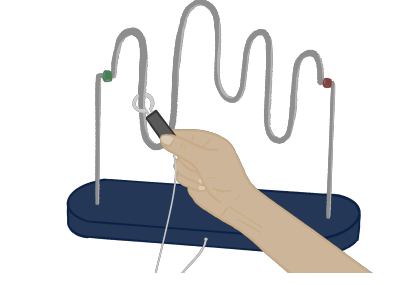
\includegraphics[width=0.8\linewidth]{1.png}
\caption{A children’s game akin to a steering task. The goal is to move a metal loop from one end of a wire to the other without the two components touching each other. Image adapted from \cite{chen2025curves}.}
\end{figure}

Building on this idea, the \textit{Curves Ahead} study investigated how curvature and path geometry influence steering performance. In their experimental setup, participants controlled a cursor and navigated it through predefined curved tunnels on a two-dimensional interface. Movement time, cursor trajectories, and error events were recorded during each trial to analyze steering behavior under different path configurations.

\begin{figure}[h]
\centering
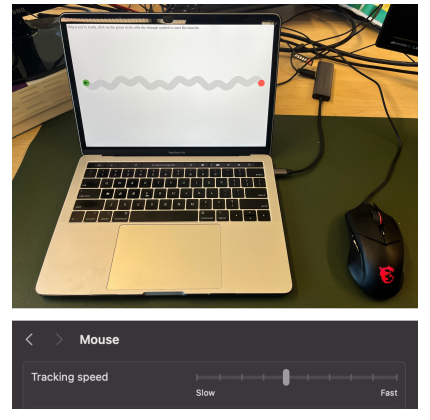
\includegraphics[width=0.8\linewidth]{2.png}
\caption{A sample of how the experimental application was designed for steering experiments in a two-dimensional environment. Image taken from the \textit{Curves Ahead} study \cite{chen2025curves}.}
\end{figure}

The study introduced several types of curved paths with different curvature and length properties. These path designs allowed researchers to systematically investigate how geometric characteristics influence steering difficulty and movement performance. The different curve configurations used in their experiment served as an important source of inspiration for the path design used in our prototype.

\begin{figure}[h]
\centering
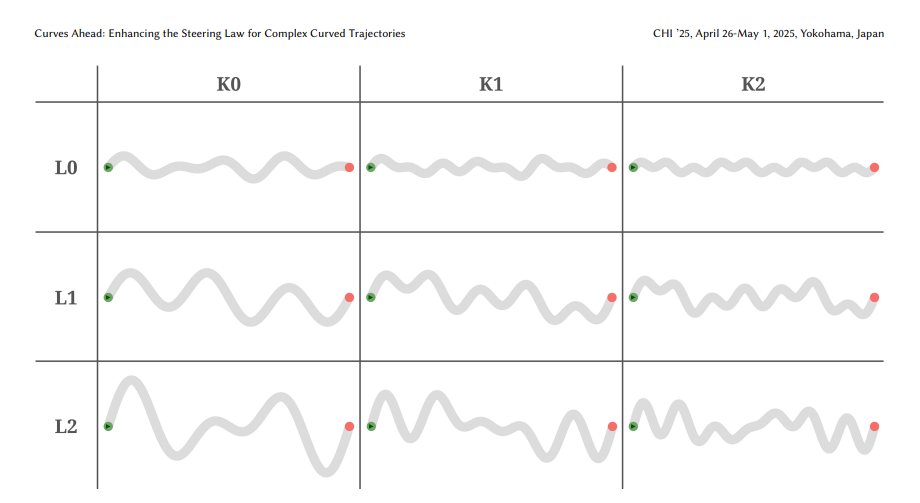
\includegraphics[width=0.8\linewidth]{3.png}
\caption{Types of curved steering paths used in the original experiment. These curve configurations inspired the steering paths implemented in our prototype. Image taken from the \textit{Curves Ahead} study \cite{chen2025curves}.}
\end{figure}

While most prior steering experiments have been conducted in two-dimensional environments, many modern interactive systems require navigation within three-dimensional spaces, such as virtual reality applications, simulation platforms, and 3D modeling environments. Motivated by this limitation, our project extends the experimental paradigm of constrained steering tasks into a three-dimensional setting.

To achieve this, we developed a high-fidelity prototype using the Unity game engine. Unity was selected primarily because three out of the four members of the project team gained practical experience with the platform during their industrial training at Battery Low Interactive. This familiarity enabled the team to rapidly prototype interactive 3D environments and implement accurate movement tracking mechanisms necessary for steering experiments.

The resulting prototype recreates the core concept of constrained path navigation while enabling steering tasks in three-dimensional space. By logging trajectory data, movement times, and steering errors, the system provides a foundation for analyzing human navigation behavior and collecting datasets that can later support Human-Centered Machine Learning (HCML) analysis.


\section{Design Goals and HCML Principles}

The design of the prototype is guided by usability and user experience goals identified during the requirements analysis phase. Since the system is intended for controlled steering experiments and human-centered machine learning (HCML) analysis, the design emphasizes reliable data collection, minimal participant burden, and clear interaction feedback. These goals ensure that participants can perform steering tasks accurately while researchers obtain high-quality behavioral data for later analysis.

\subsection{Usability Goals}

The usability goals of the system focus on ensuring that participants can interact with the experimental environment easily and consistently while minimizing the likelihood of interface-related errors.

\textbf{Effectiveness.} The system should allow participants to successfully complete steering trials within the predefined paths without requiring external assistance. The interface is therefore designed to clearly display the steering tunnel, start and end points, and the participant’s cursor or object position. This visual clarity helps users maintain control and complete tasks reliably.

\textbf{Efficiency.} Experimental systems must allow researchers to configure and run trials quickly. The prototype therefore provides a streamlined workflow where steering tasks can be launched with minimal setup time. Clear interface elements and automated logging mechanisms reduce the time required to begin experiments and collect data.

\textbf{Learnability.} Since participants may be unfamiliar with steering experiments, the system includes a short tutorial phase where users can practice navigating along sample paths. This allows participants to understand the controls and interaction mechanics before entering the actual experiment trials.

\textbf{Error Tolerance.} Steering tasks may involve occasional boundary violations or temporary loss of control. The prototype is designed to record these events without interrupting the experiment workflow. Participants can continue navigating even after minor errors, ensuring that data collection proceeds smoothly.

\textbf{Data Integrity.} Accurate behavioral data is critical for HCML analysis. The system therefore records trajectory coordinates, movement times, and boundary violations with synchronized timestamps. Logging mechanisms ensure that no trajectory data is lost during trials.

\subsection{User Experience Goals}

Beyond basic usability, the prototype is designed to create a clear and predictable user experience that supports participant confidence and reduces cognitive load during experiments.

First, the interface aims to provide a focused and distraction-free environment where the steering path and navigation task remain visually prominent. This helps participants concentrate on the steering task without unnecessary interface complexity.

Second, the system provides immediate visual feedback regarding cursor position and path boundaries. When participants approach or exit the steering tunnel, the system can record and optionally visualize these events, helping users better understand their performance during the task.

Third, the experimental workflow is structured to be predictable and easy to follow. Participants move through clearly defined phases including practice trials, experimental trials, and breaks between blocks. This structured interaction flow helps maintain participant engagement and reduces fatigue during longer experiment sessions.

Finally, the interface is designed to minimize cognitive load by using simple control mechanisms and consistent visual layouts across trials. This ensures that the recorded performance reflects user steering ability rather than confusion caused by interface complexity.

\subsection{Human-Centered Machine Learning Principles}

The prototype is also designed according to Human-Centered Machine Learning (HCML) principles, which emphasize the alignment of machine learning systems with human needs, transparency, and reliable data collection.

\textbf{Transparency.} The system clearly communicates the structure of each trial and the user's progress during the experiment. Participants can easily identify the path they must navigate and understand when a trial begins or ends.

\textbf{Explainability.} Although the current prototype focuses on data collection rather than automated decision-making, the interface is designed so that the collected behavioral data can be easily interpreted and analyzed by researchers. Clear visual representations of steering paths and trajectories help explain how performance metrics are generated.

\textbf{Reliability.} For machine learning analysis, the quality of collected data is essential. The system therefore prioritizes stable input tracking, synchronized logging of trajectory data, and consistent experimental conditions across trials.

\textbf{Human Oversight.} Researchers retain full control over experiment configuration, trial execution, and data collection. The system functions as a tool that supports researchers in studying human steering behavior rather than replacing human judgment or decision-making.

By integrating these usability, user experience, and HCML design principles, the prototype provides a reliable experimental environment for studying steering behavior in three-dimensional interaction tasks and generating datasets suitable for future machine learning analysis.
\section{Conceptual Design of the System}

\subsection{System Overview}

The proposed system is an experimental platform designed to evaluate human steering performance in complex three-dimensional environments. The primary purpose of the system is to provide a controlled interactive environment where users can navigate an object through predefined 3D paths while their movement behavior is recorded for later analysis. The collected data can then be used to study human steering performance and support Human-Centered Machine Learning (HCML) models that analyze navigation behavior in constrained environments.

The system is implemented as a high-fidelity prototype in the Unity game engine and focuses on a vertical slice of functionality that demonstrates the core experimental workflow. Users interact with the system by steering a cursor or object through curved tunnels or paths while the system records trajectory coordinates, movement time, and boundary violations.

The primary users of the system are researchers and students working in Human–Computer Interaction (HCI), interaction design, or machine learning who wish to conduct controlled steering experiments. Participants performing the steering tasks represent the secondary user group, as they interact directly with the experimental environment during data collection sessions.

The key functionalities of the system include the generation of steering paths, execution of navigation trials, real-time visualization of the steering task, and automatic logging of user interaction data. Together, these components form a platform that supports experimental studies of human navigation behavior in three-dimensional interactive environments.

\subsection{Conceptual Model}

The conceptual model of the system is based on a task-oriented interaction framework in which users navigate a virtual object through constrained spatial paths. The system presents a 3D tunnel or trajectory that represents the steering path. Participants control a movable object and attempt to traverse the path from start to finish without crossing its boundaries.

From the user's perspective, the interaction model is straightforward: the participant observes the path, initiates a trial, and navigates through the tunnel while maintaining control of the object. If the object exits the path boundaries, the system logs the event but allows the participant to continue the trial. This design ensures uninterrupted interaction and consistent data collection.

Internally, the system manages several components that support this interaction process. The environment module renders the 3D paths and experimental interface. The interaction module captures user input and updates the object's movement within the environment. The logging module continuously records trajectory coordinates, timestamps, and error events during each trial. These modules work together to translate user actions into measurable behavioral data.

By structuring the system around these components, the conceptual model ensures that users can clearly understand the relationship between their actions and the outcomes produced by the system. Such clarity is essential for experimental environments where consistent user behavior and reliable data collection are required.


\subsection{Human--ML Interaction Model}

The prototype is designed to support a Human–Machine Learning (Human--ML) interaction workflow in which human steering behavior forms the primary source of data for subsequent machine learning analysis. In this model, the human participant performs steering tasks within the experimental environment, while the system records detailed behavioral data that later serve as input for analytical and machine learning models.

During each trial, the participant navigates an object through a predefined three-dimensional path while the system continuously records trajectory coordinates, movement time, and boundary violation events. These interaction traces represent the behavioral dataset generated through human interaction with the system. The reliability and completeness of this collected data are therefore critical for meaningful downstream analysis.

After the data collection phase, the recorded trajectories and performance metrics can be analyzed using two complementary approaches. First, the experimental results can be compared with established analytical models such as the Steering Law, which relates movement time to path length and width. Second, machine learning models can be applied to the collected dataset to identify patterns in steering behavior, predict task difficulty, or model the influence of geometric path properties such as curvature and length.

Within this framework, the human user remains the central actor responsible for generating behavioral data through interaction with the system, while machine learning methods function as analytical tools that interpret and model the observed behavior. This Human--ML interaction paradigm aligns with Human-Centered Machine Learning (HCML) principles by emphasizing the role of human performance data as the foundation for computational analysis and modeling.

\section{Prototype Design Methodology}

\subsection{Prototyping Approach}

A vertical prototyping approach was employed to construct the high-fidelity 3D steering evaluation system. Vertical prototyping emphasizes full implementation of selected features rather than shallow coverage of all possible functionalities, allowing the team to focus on critical interaction and data collection components. The design process began with brainstorming sessions to outline key system goals, identify essential user interactions, and define the experimental tasks. 

Following this, sketches and wireframes were developed to visualize interface layouts, 3D path configurations, and control schemes. Iterative design cycles were used to refine both interaction mechanics and visual presentation, informed by continuous internal testing and review. Particular attention was given to path navigation, feedback mechanisms, and real-time trajectory logging to ensure accurate data collection for downstream Human-Centered Machine Learning (HCML) analysis. This approach allowed the team to rapidly implement and evaluate functional components, ensuring usability and experimental validity before full-scale development.

\subsection{Tools and Technologies}

The prototype was implemented in \textbf{Unity 3D}, leveraging its physics engine, flexible input system, and visualization capabilities for three-dimensional environments. Unity allowed precise control over object movement, collision detection, and 3D path rendering. C\# scripts were used to implement core functionalities, including steering task mechanics, boundary detection, trajectory logging, and trial management. Additional tools included the Unity Editor for scene construction, the Input System for handling various input devices, and data serialization libraries for exporting interaction traces to JSON formats suitable for subsequent HCML analysis.

\subsection{Human--ML Behavior Simulation}

While the prototype does not include autonomous AI-driven assistance during trials, it is designed to facilitate Human--ML interaction by generating high-quality datasets for machine learning analysis. The system simulates controlled experimental conditions, including path constraints, trial timing, and error feedback, enabling consistent and reproducible data collection. After each trial, recorded trajectories and performance metrics serve as input for both analytical models (e.g., Steering Law) and machine learning pipelines. This simulation ensures that the interaction between human behavior and computational analysis can be rigorously evaluated, laying the foundation for future predictive modeling and pattern discovery in steering tasks.
\section{Prototype Artifacts and Interface Design}

\subsection{Wireframes and Sketches}

Early-stage wireframes were developed to explore the layout and interaction flow of the proposed system prior to full implementation. At this stage, the emphasis was on structural organization rather than visual styling, allowing rapid iteration and refinement of key interaction elements.

As shown in Figure~\autoref{fig:wireframes}, the wireframes illustrate the primary components of the interface. These include the 3D simulation area, where users perform the steering task; the control panel, which provides adjustable parameters such as rope length, radius, and curve coefficients; the status bar, which displays task instructions, progress, and feedback; and the top information bar, which presents elapsed time and control hints.

The figure also presents multiple system states and user interactions. The initial frames depict the default interface with minimal controls visible, while subsequent frames demonstrate the expanded control panel and the active task state during simulation. Additional frames further illustrate feedback conditions, such as task progression and paused states.

These wireframes helped refine the spatial arrangement of interface elements, ensure a clear and intuitive interaction flow, and maintain a balance between functionality and cognitive load. By visualizing different stages of interaction, the design enables users to easily understand controls, monitor performance, and remain focused on the steering task without unnecessary distractions.

\begin{figure}[htbp]
    \centering

    \begin{subfigure}{0.3\textwidth}
        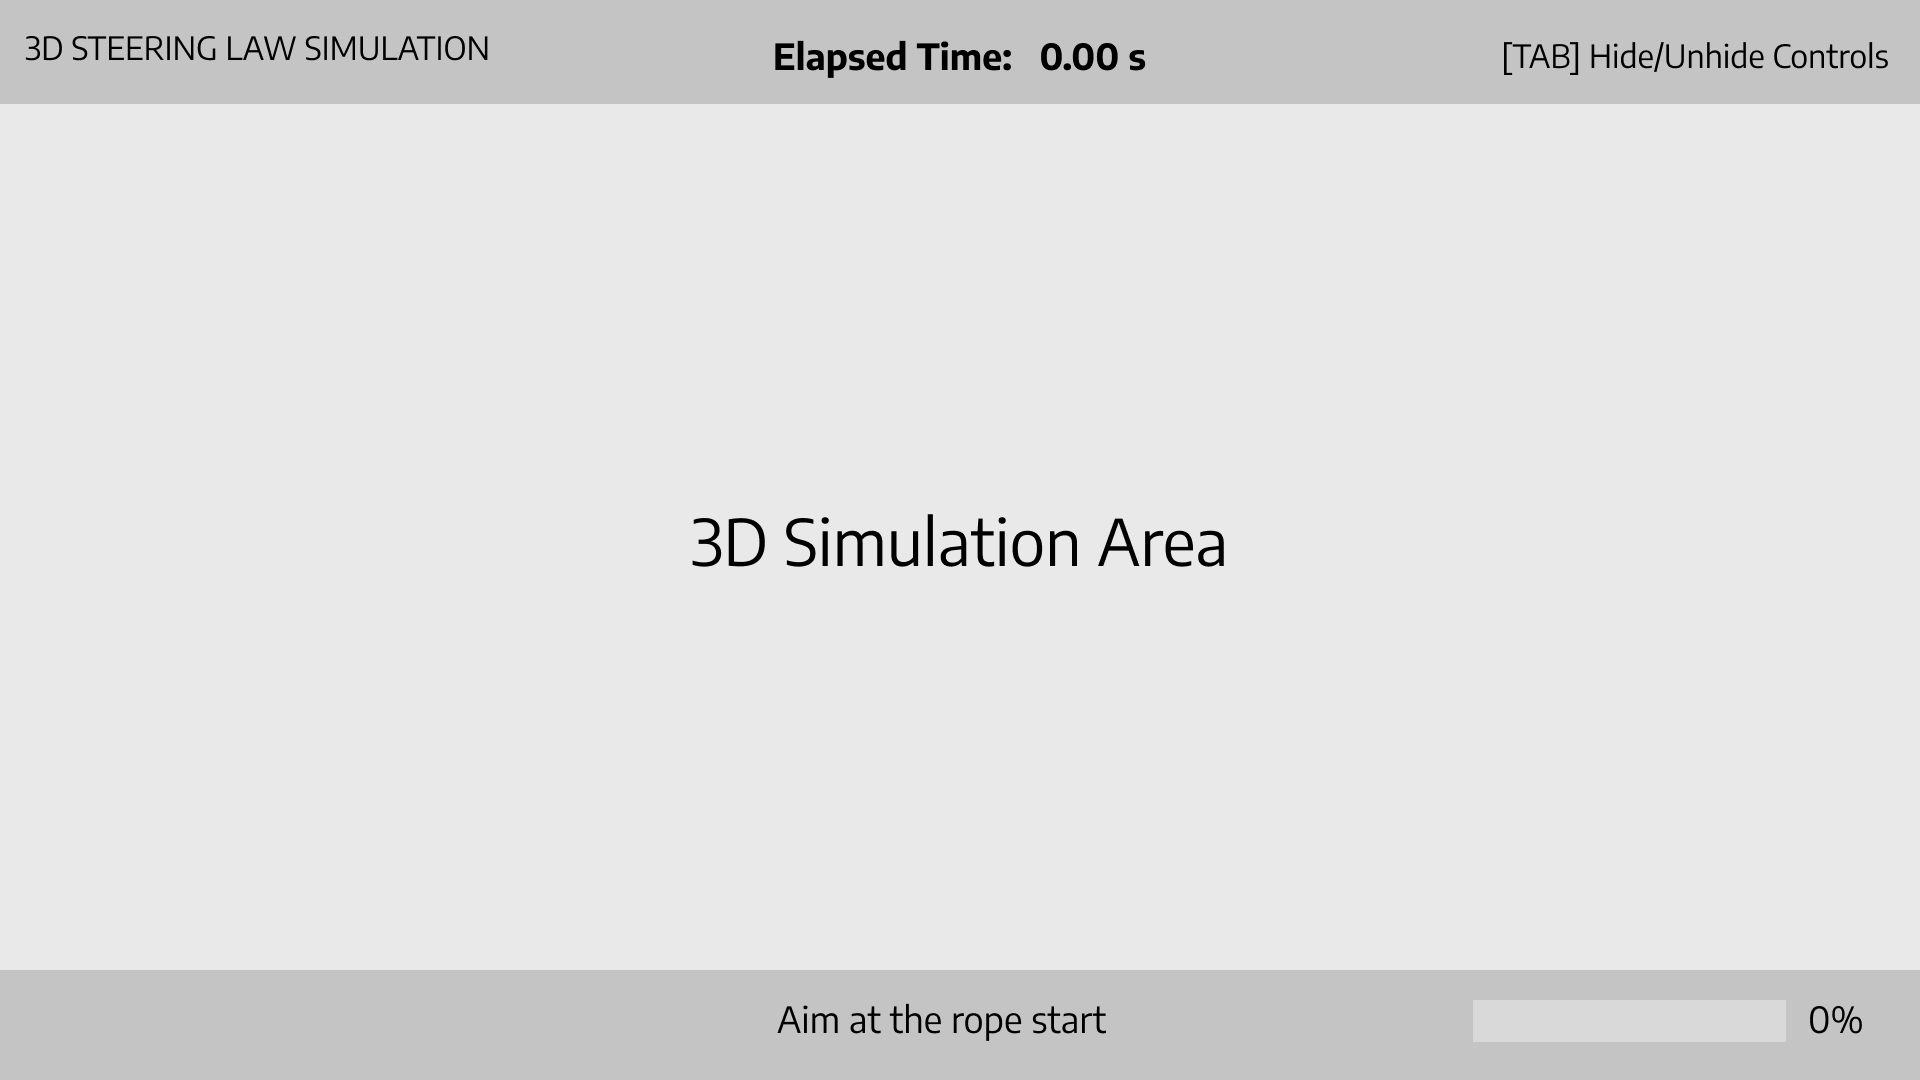
\includegraphics[width=\linewidth]{Wireframes/Frame1.png}
        \caption{Default interface}
    \end{subfigure}
    \hfill
    \begin{subfigure}{0.3\textwidth}
        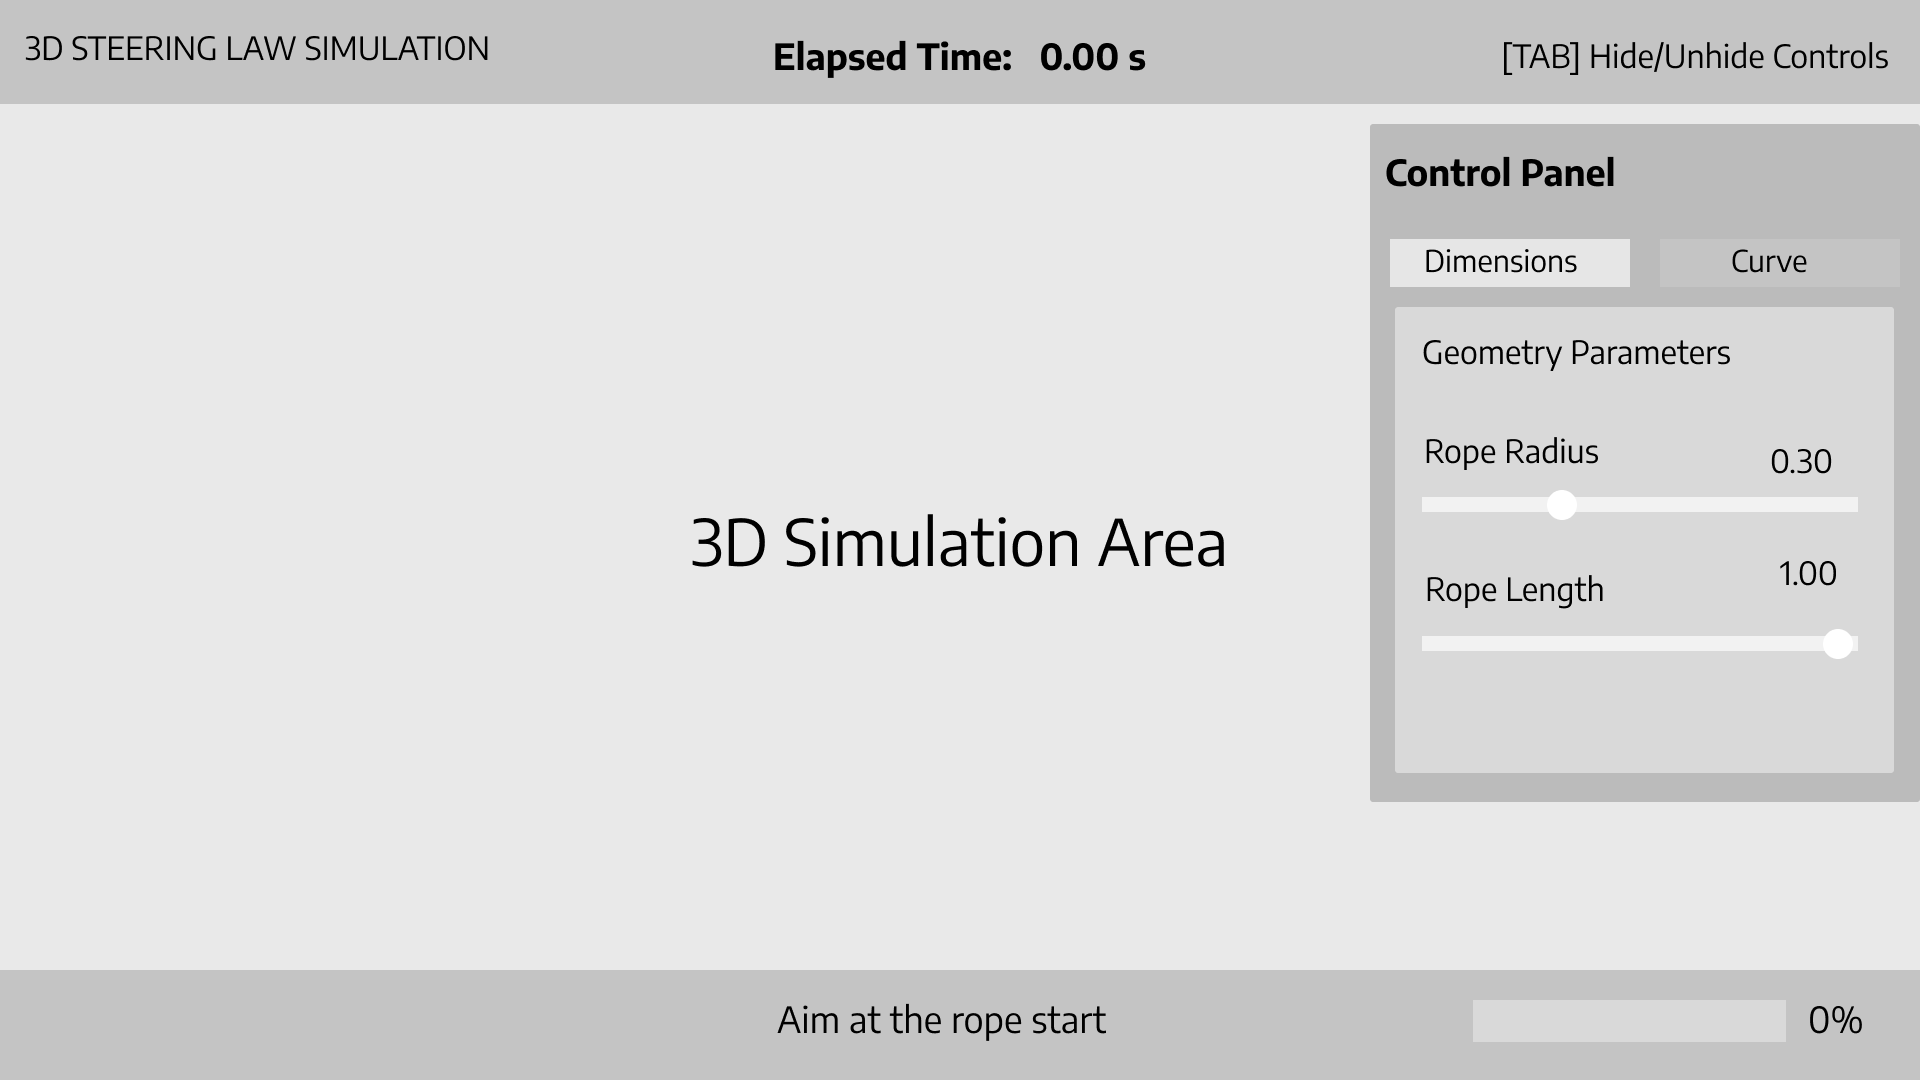
\includegraphics[width=\linewidth]{Wireframes/Frame2.png}
        \caption{Control panel opened}
    \end{subfigure}

    \medskip

    \begin{subfigure}{0.3\textwidth}
        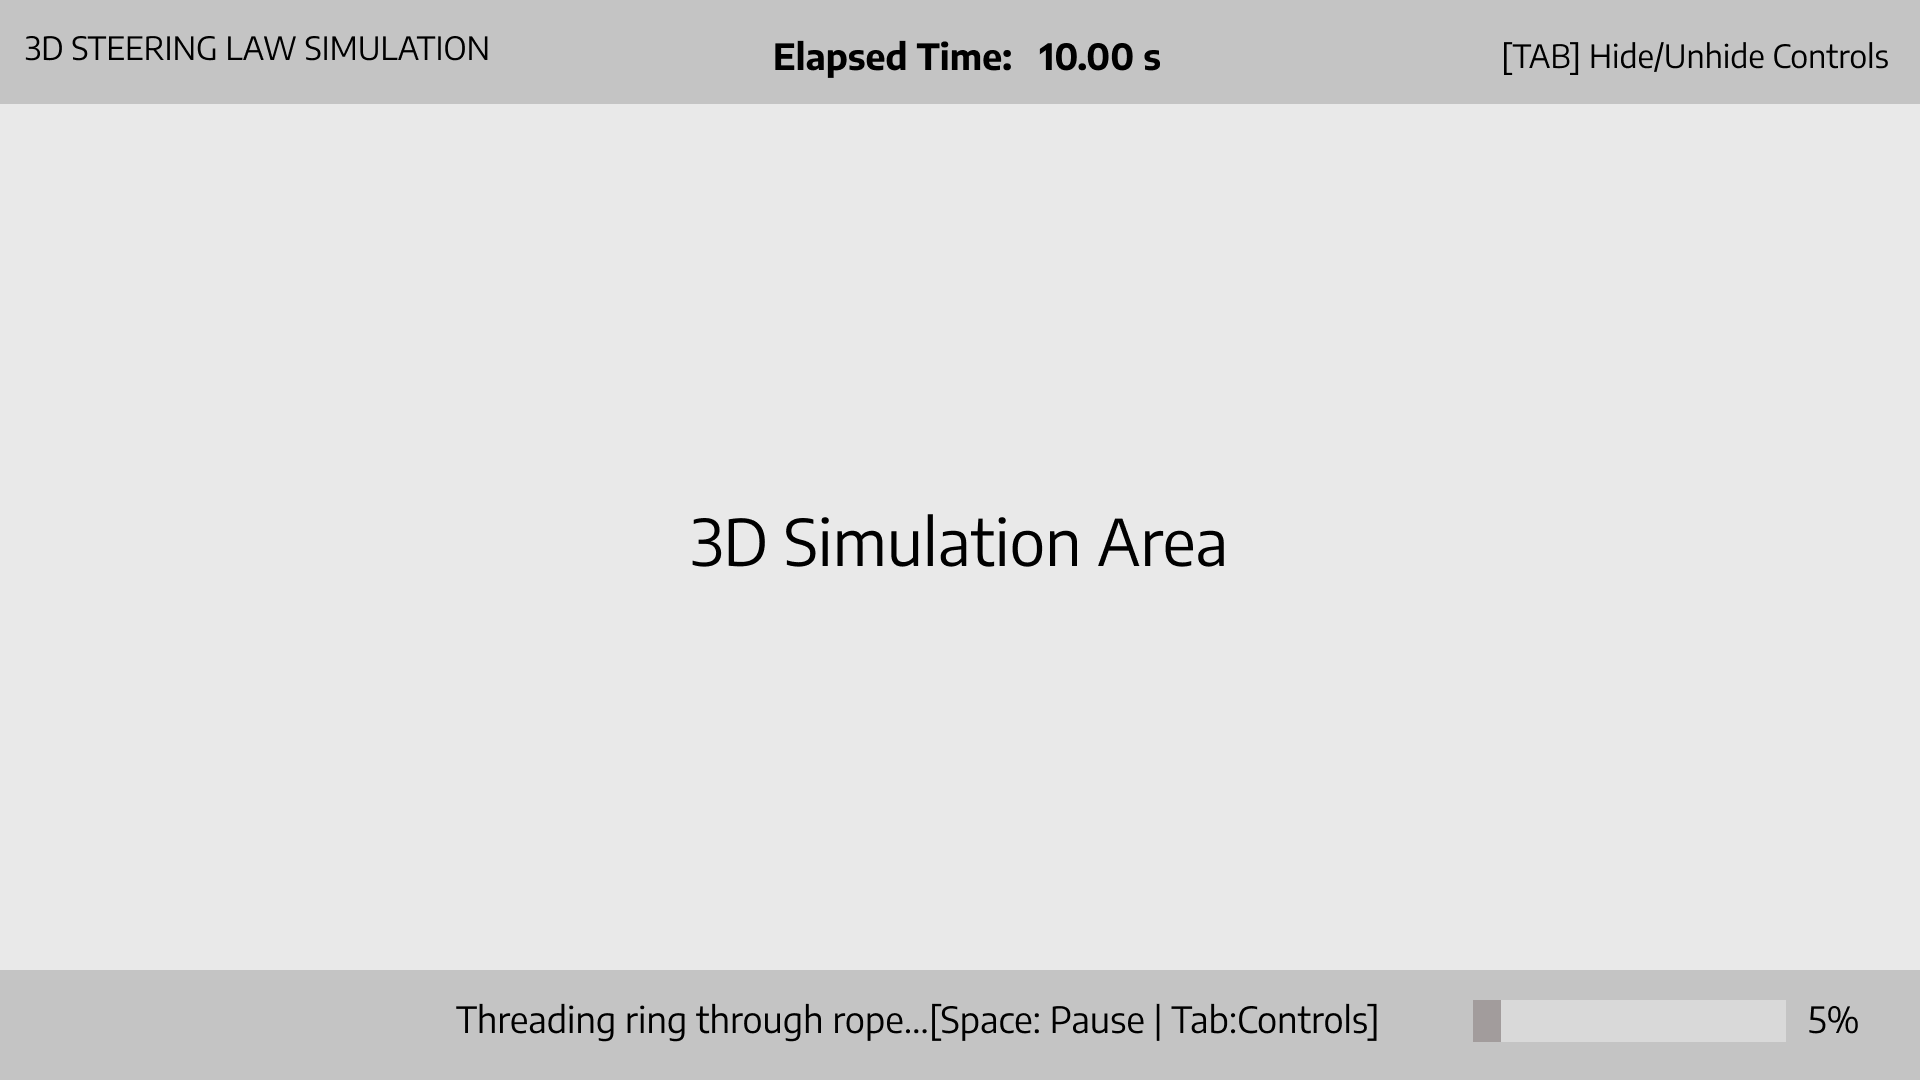
\includegraphics[width=\linewidth]{Wireframes/Frame3.png}
        \caption{Task in progress}
    \end{subfigure}
    \hfill
    \begin{subfigure}{0.3\textwidth}
        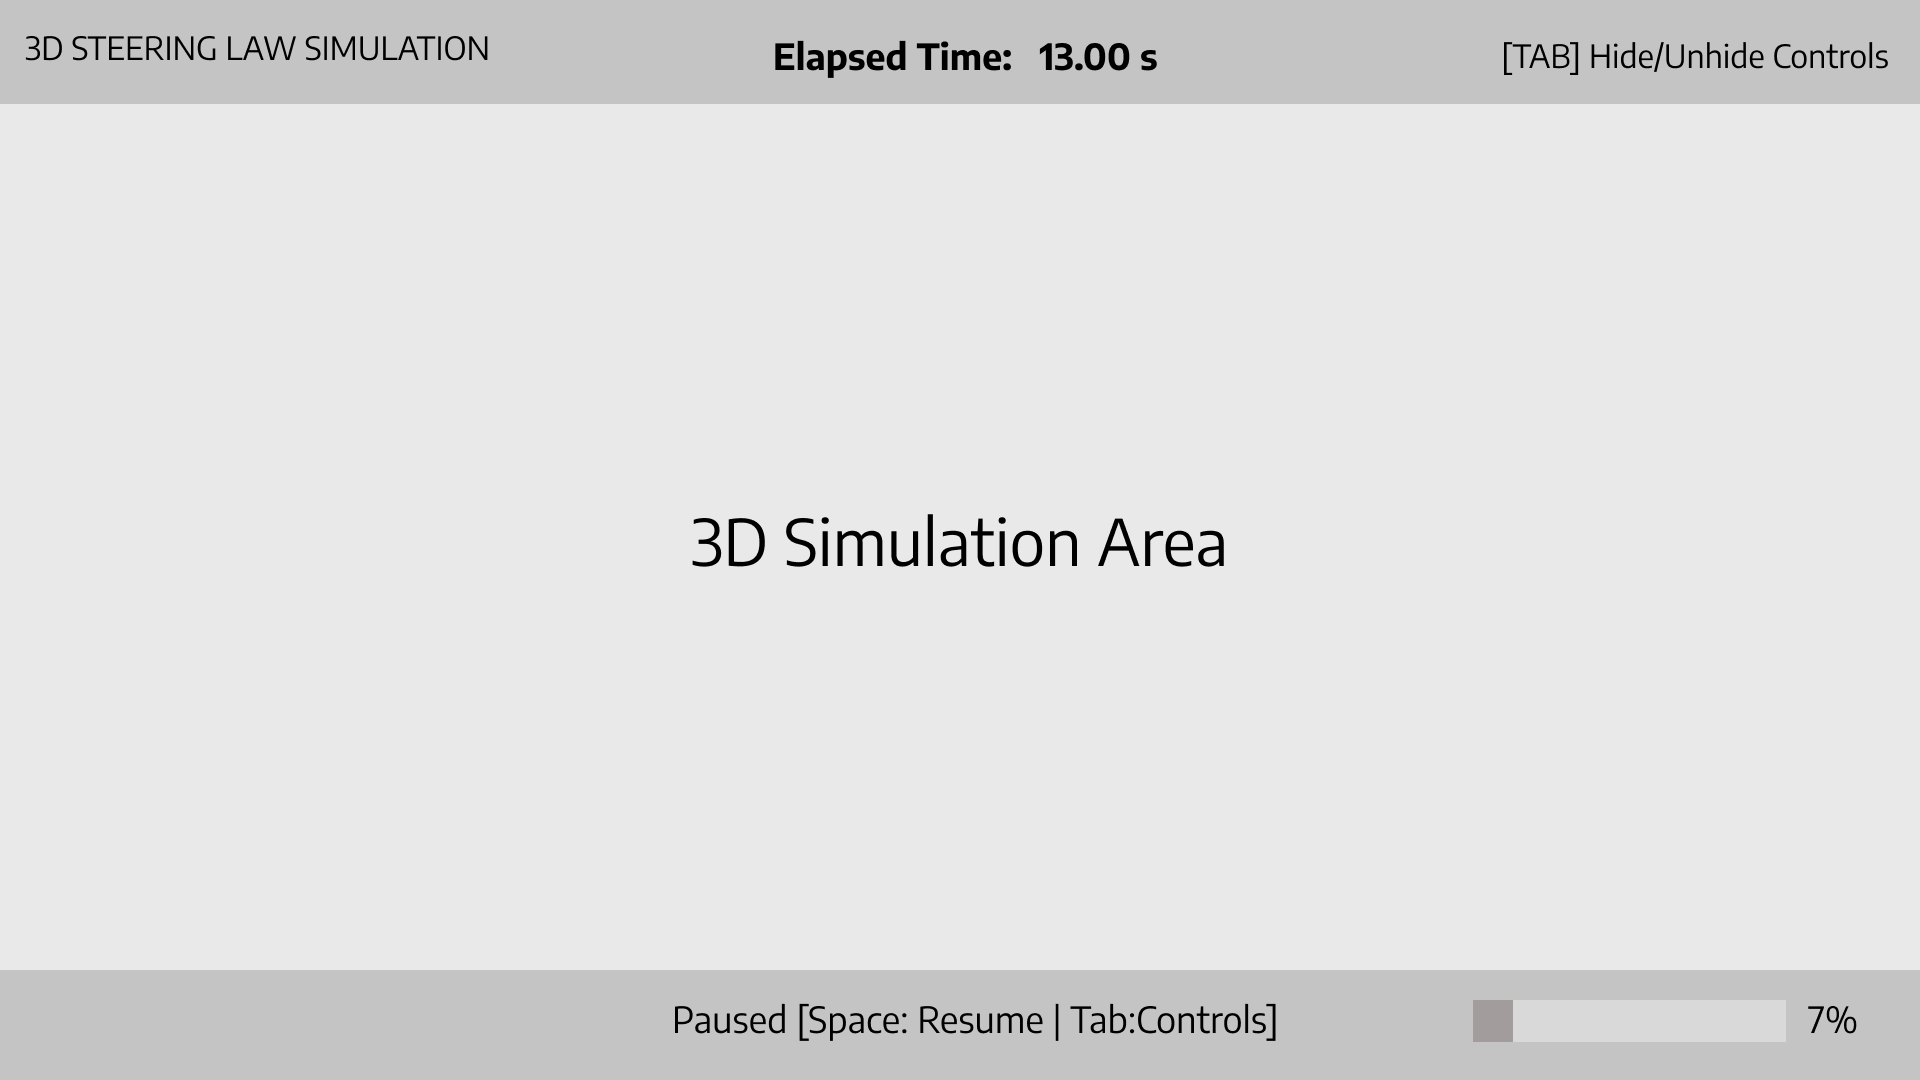
\includegraphics[width=\linewidth]{Wireframes/Frame4.png}
        \caption{Paused state}
    \end{subfigure}

    \caption{Wireframes showing different states of the system interface.}
    \label{fig:wireframes}
\end{figure}

\subsection{Interface Screens}

The interface is designed around a set of core screens that support different stages of user interaction while maintaining a consistent visual structure (see~\autoref{fig:all_screens}). The central element across all screens is the 3D simulation area, which remains the primary focus of user attention.

The default screen, shown in~\autoref{start}, presents a minimal interface. Here, the user sees the rope path, the controlled object or ring, and a target indicator. Only essential information is displayed, including the top information bar showing elapsed time and a control hint (e.g., toggling the control panel), and the bottom status bar providing brief instructions such as “Aim at the rope start.” This minimal design reduces cognitive load and helps users quickly understand the task environment without distraction.

The task-in-progress screen (\autoref{task_in_progress} and \autoref{changed_settings}) introduces dynamic feedback as the user begins interaction. The controlled object moves along or toward the rope path, which is visualized as a smooth, continuous 3D curve, while the status bar updates to reflect task progress. During this stage, the status bar shows: "Threading ring through rope... [Space: Pause | Tab: Controls]." This communicates both the current action and the available control options, guiding user actions and maintaining engagement. The progress bar, showing percentage completion, is located at the bottom-right corner. This placement ensures visibility of real-time feedback without obstructing the main simulation area, guiding user actions and maintaining engagement.

The control panel screen appears when the experiment setter or researcher activates the side panel by pressing TAB on the keyboard (\autoref{change_radius}). This hide/unhide mechanism reflects key HCI principles, particularly progressive disclosure, user control and freedom: advanced controls are kept out of view by default to reduce visual clutter, but remain instantly accessible when needed. Activating the control panel freezes the simulation and resets it to its initial state to ensure that any parameter changes (such as curve shape, rope length, or radius) are applied consistently from a known starting point. This prevents inconsistencies that could arise if changes were made mid-task. The panel is positioned on the right side and uses a semi-transparent/dimmed background to avoid completely blocking the simulation. Sliders and labeled fields allow intuitive interaction and precise control while still observing the effects of adjustments in real time.

The parameter-adjustment state (e.g., changing radius or curve properties) emphasizes immediate visual feedback. As the experiment setter or researcher modifies values in the control panel, corresponding changes are reflected directly in the 3D environment, particularly in the rope geometry. This tight coupling between input and visual response supports exploratory interaction and improves understanding of system behavior.

The paused screen in ~\autoref{paused} clearly communicates that the simulation is temporarily halted when the user presses the Space key. Visual indicators (such as a pause label or status message) inform the user that input is inactive while preserving the current state of the scene. This prevents confusion and allows users to resume the task seamlessly.

When a task is finished, the status bar displays “Completed”, and the timer stops, clearly signaling to the user that the objective has been achieved.

Across all screens, the layout follows a consistent hierarchy: the simulation area occupies the center, controls are placed peripherally and can be toggled, and informational elements are anchored at the top and bottom. This separation ensures that critical task-related visuals remain unobstructed. Design decisions prioritize clarity, real-time feedback, minimal distraction, and predictable behavior, enabling users to focus on the steering task while having access to necessary controls and information when needed.


\begin{figure*}[htbp]
    \centering

    % Row 1
    \begin{subfigure}[t]{0.3\textwidth}
        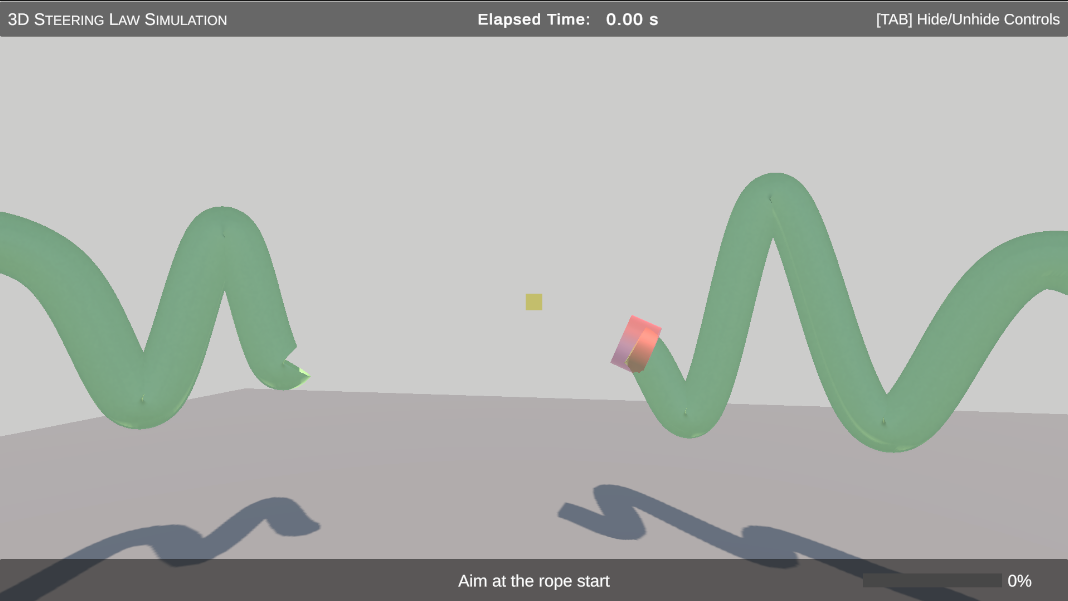
\includegraphics[width=\linewidth]{UserInterface/Start.png}
        \caption{Start Screen}
        \label{start}
    \end{subfigure}
    \hfill
    \begin{subfigure}[t]{0.3\textwidth}
        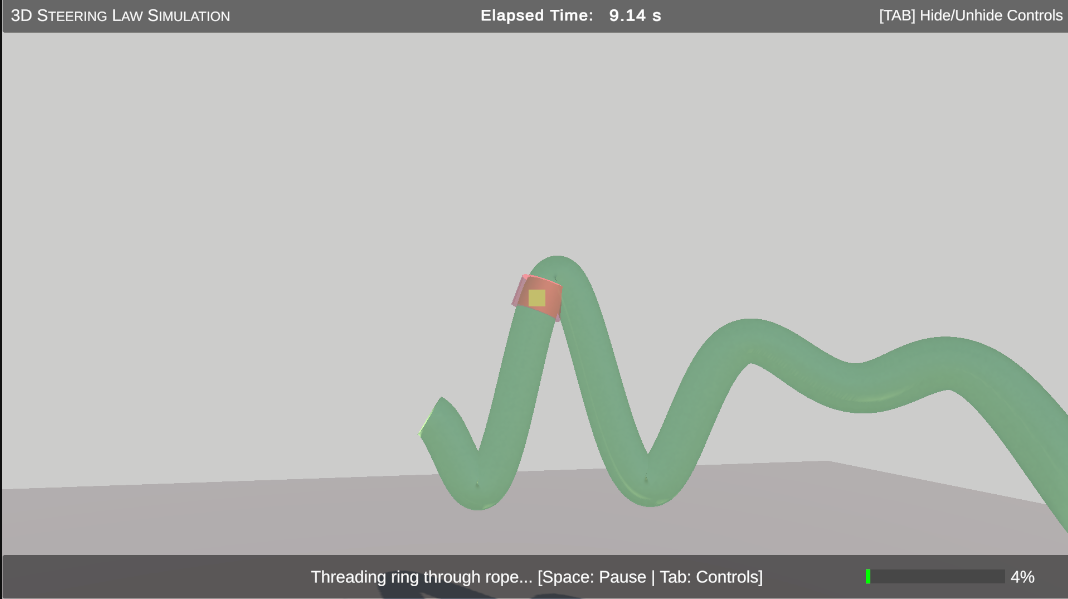
\includegraphics[width=\linewidth]{UserInterface/Task in progress1.png}
        \caption{Task in progress}
        \label{task_in_progress}
    \end{subfigure}
    \hfill
    \begin{subfigure}[t]{0.3\textwidth}
        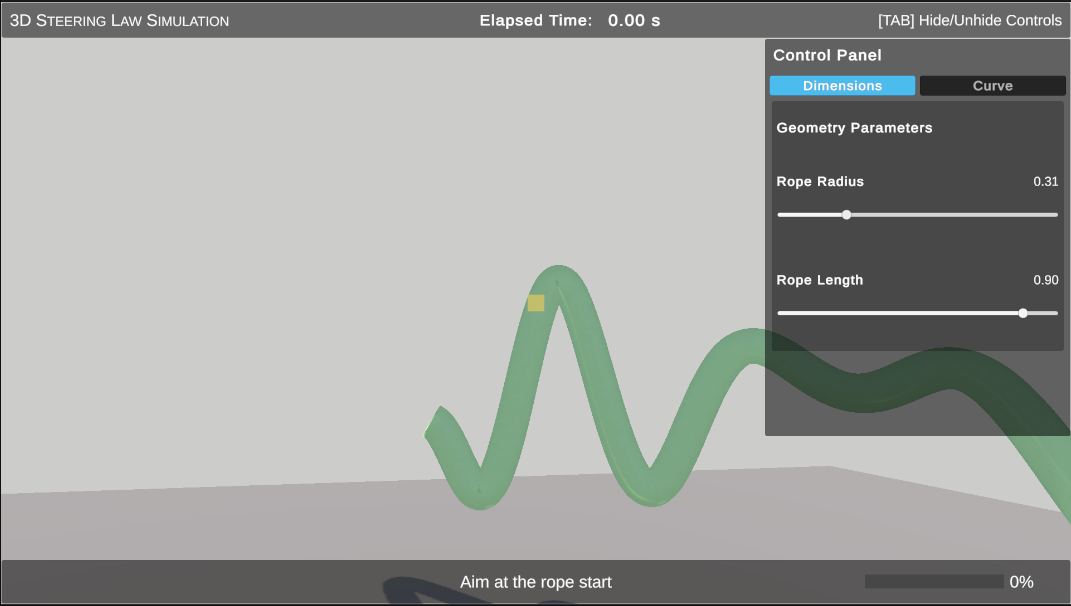
\includegraphics[width=\linewidth]{UserInterface/Radius.png}
        \caption{Control panel opened, radius of rope is changed}
        \label{change_radius}
    \end{subfigure}

    \medskip

    % Row 2
    \begin{subfigure}[t]{0.3\textwidth}
        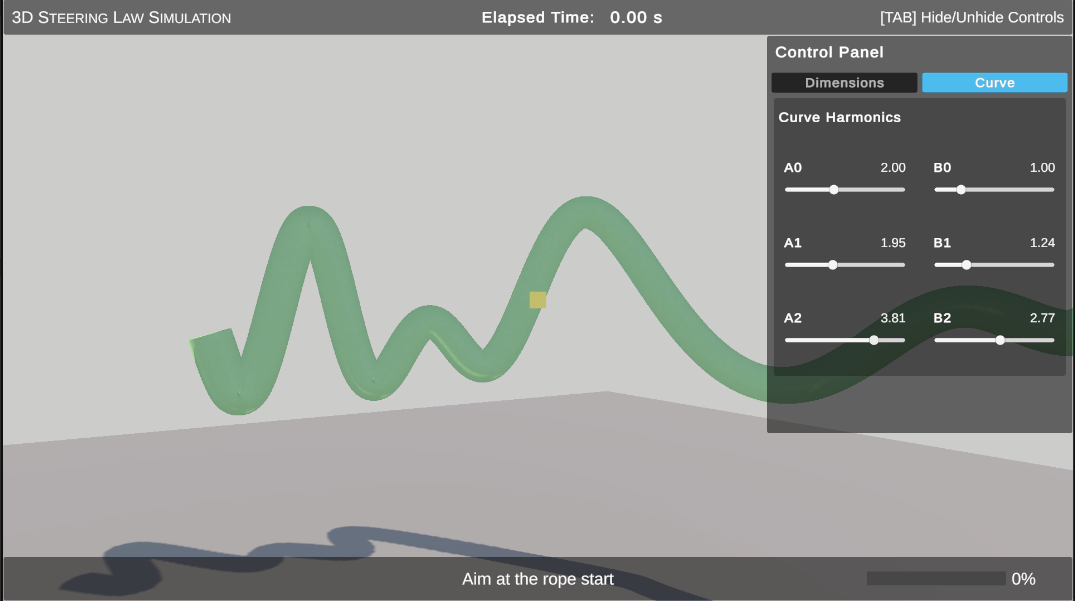
\includegraphics[width=\linewidth]{UserInterface/Curve.png}
        \caption{Curve properties in Curve tab of the control panel are changed}
        \label{change_curve}
    \end{subfigure}
    \hfill
    \begin{subfigure}[t]{0.3\textwidth}
        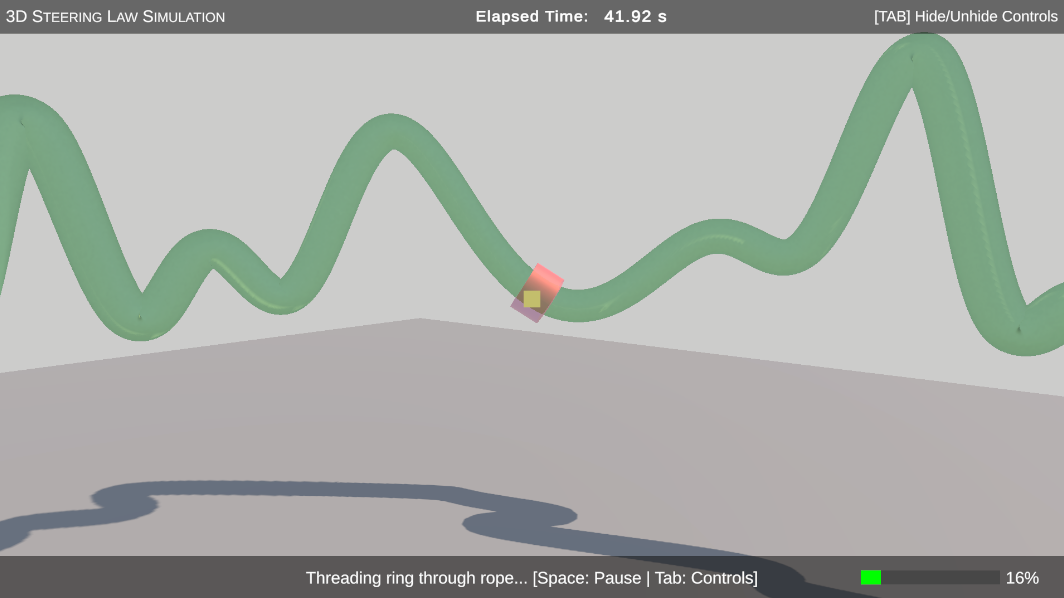
\includegraphics[width=\linewidth]{UserInterface/Task in progress.png}
        \caption{Task in progress with changed settings}
        \label{changed_settings}
    \end{subfigure}
    \hfill
    \begin{subfigure}[t]{0.3\textwidth}
        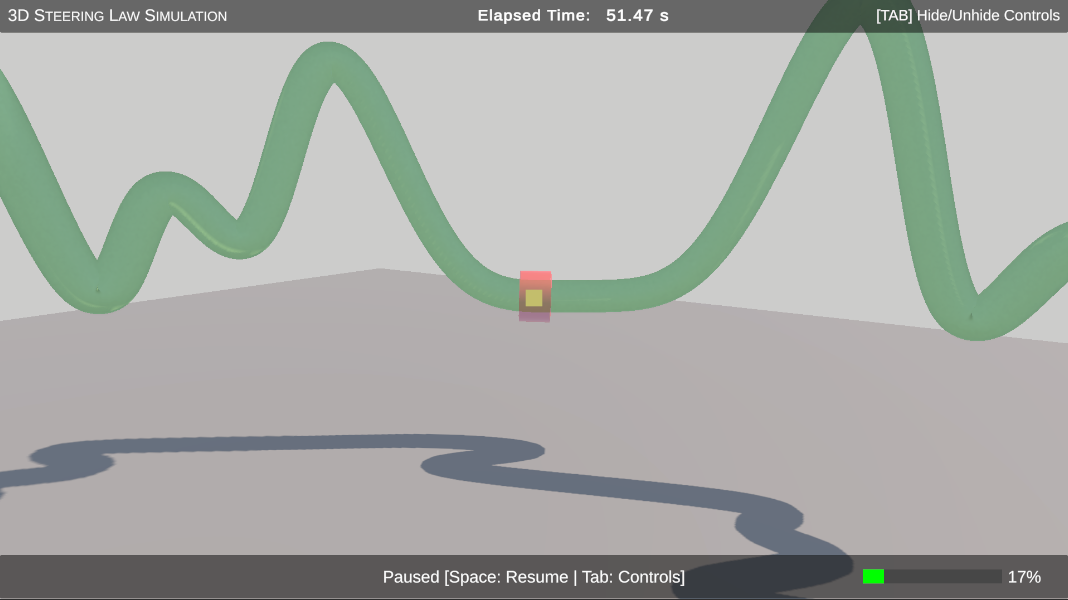
\includegraphics[width=\linewidth]{UserInterface/Paused.png}
        \caption{Simulation paused by user}
        \label{paused}
    \end{subfigure}

    \caption{System interface across different states.}
    \label{fig:all_screens}
\end{figure*}

\subsection{Storyboards and Interaction Scenarios}

Storyboards were created to illustrate realistic interaction scenarios between the researcher and the participant during the experimental process. These scenarios help visualize how the proposed system will be used in practice and how different actors interact with the prototype. The storyboard represents the overall workflow of the experiment, beginning with the preparation of the VR setup by the researcher, followed by the participant performing the steering task using a VR headset and handheld controllers within the virtual environment.

During the task, the system records movement trajectories, completion time, and boundary violations while the researcher supervises the experiment and monitors the data collection process. After the participant completes the trials, the recorded interaction data are collected and stored for further analysis. These data will later be analyzed using both analytical steering models and machine learning approaches to better understand user performance in complex curved trajectories.

The storyboard reflects the previously defined personas: the \textit{participant}, who provides the interaction data by performing steering tasks, and the \textit{researcher}, who prepares the experimental environment, oversees the session, and collects the resulting data for subsequent analysis.

\begin{figure}[h]
\centering
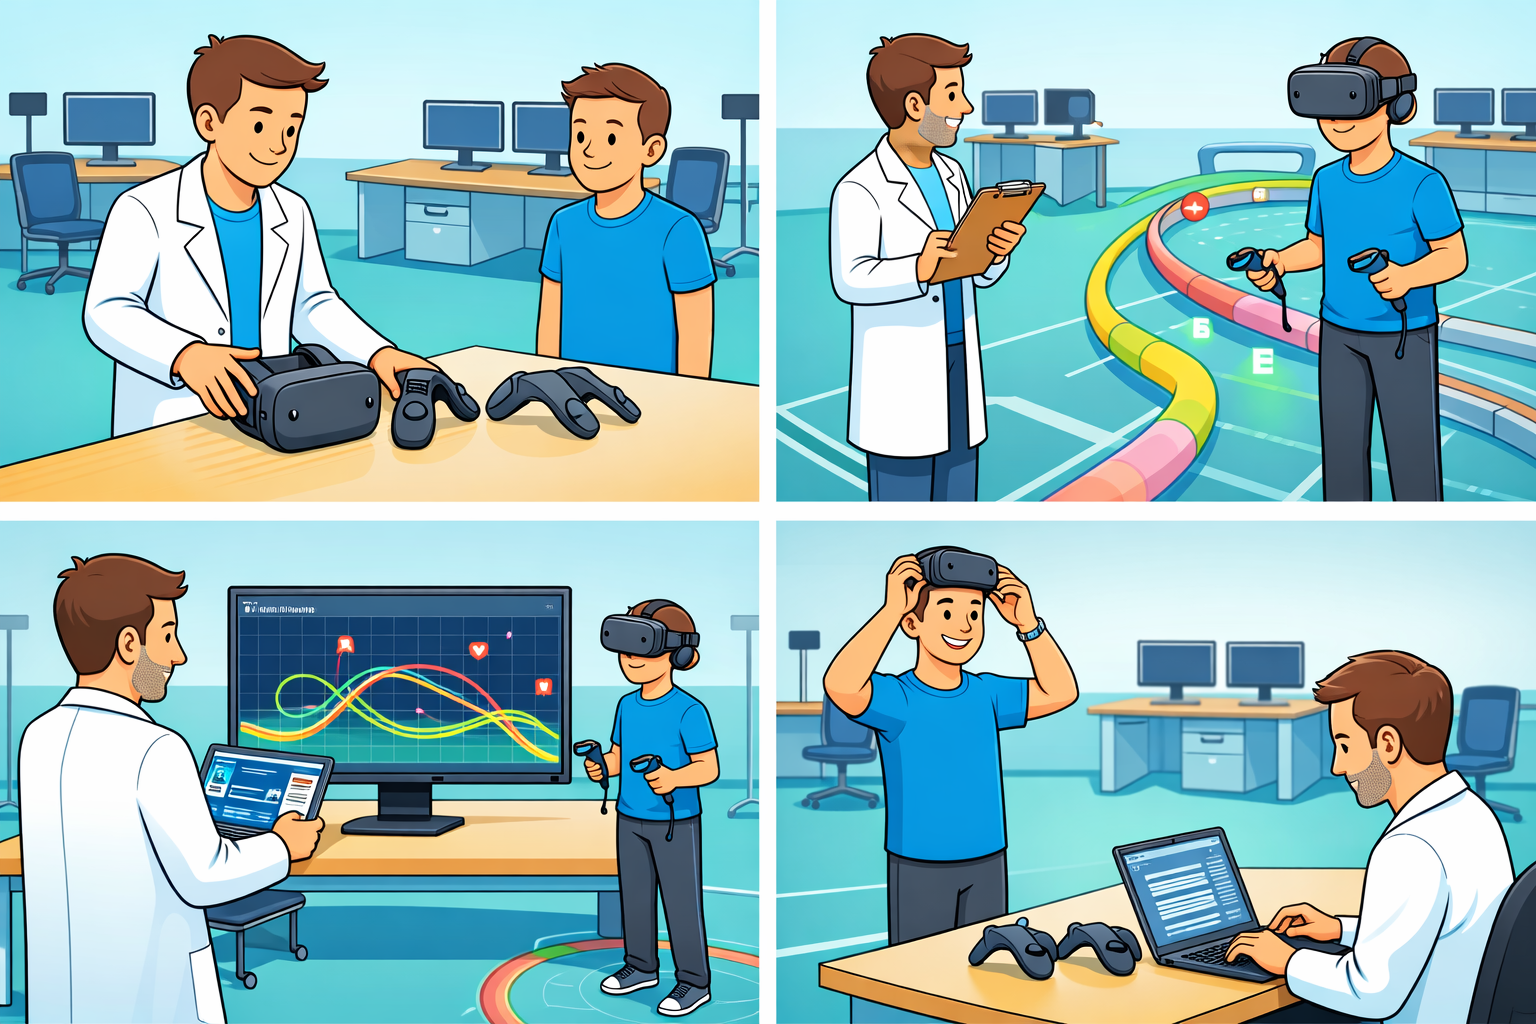
\includegraphics[width=0.9\linewidth]{storyboard.png}
\caption{Storyboard illustrating the experimental workflow. The sequence shows the researcher preparing the VR setup, the participant performing the steering task using a VR headset and controllers, the monitoring of movement trajectories and errors during the task, and the researcher collecting the recorded data for subsequent analysis and modeling.}
\end{figure}
\section{User Interaction and Task Flow}

\subsection{Task Scenarios}

The system is designed primarily for controlled experimental studies investigating human steering behavior in three-dimensional environments. Two main user roles interact with the system: the researcher and the participant.

The researcher is responsible for configuring the experimental setup, preparing the VR environment, and supervising the data collection process. Before the experiment begins, the researcher launches the Unity-based application, selects the appropriate experimental configuration, and ensures that the VR headset and controllers are functioning correctly.

The participant performs the steering task within the virtual environment. While wearing the VR headset and holding the controllers, the participant navigates through predefined three-dimensional curved trajectories. The objective is to follow the path as accurately and smoothly as possible while minimizing deviations from the tunnel boundaries. During each trial, the system records movement trajectories, completion time, and boundary violations.

After completing the assigned trials, the collected interaction data are automatically stored and made available for later analysis.

\subsection{Interaction Flow}

The interaction flow of the system follows a structured sequence designed to ensure consistent experimental conditions and reliable data collection.

First, the researcher prepares the experimental environment by launching the application and verifying the VR equipment. The participant is then introduced to the experiment and given brief instructions about the steering task and the controls used for movement.

Next, the participant wears the VR headset and holds the controllers. Once the experiment begins, a predefined curved path appears in the virtual environment. The participant navigates through this path by moving within the VR space using the controllers. The system continuously tracks the participant’s position relative to the path and records trajectory data throughout the trial.

If the participant deviates from the path boundaries, the system logs the event as an error but allows the participant to continue the task without interruption. After completing each trial, the system automatically proceeds to the next trajectory according to the experimental design.

When all trials are completed, the participant exits the VR environment and the researcher stores the recorded data for further analysis.

\subsection{Human–ML Interaction Flow}

Although machine learning does not directly assist the participant during the experiment, it plays an important role in the post-experiment analysis phase. The collected trajectory data, movement times, and error measurements serve as input for both analytical models of steering behavior and machine learning models.

After data collection, the researcher processes the recorded interaction logs and extracts relevant performance metrics. These data are then used to fit analytical steering models and train machine learning models that aim to better understand user performance in complex three-dimensional curved trajectories.

Through this human–machine learning interaction process, the experimental system enables the generation of empirical datasets that support the development and evaluation of predictive models for human steering behavior. The insights obtained from these models can contribute to improved interaction design and a deeper understanding of human motor control in virtual environments.

\section{Implementation Details}

\subsection{Tools and Platforms}

The prototype system was implemented using the Unity game engine, which provides a flexible environment for developing interactive three-dimensional applications. Unity was selected because of its strong support for real-time rendering, physics simulation, and compatibility with virtual reality (VR) devices. Additionally, several members of the development team had prior experience with Unity from their internship at Battery Low Interactive, which allowed the team to rapidly prototype and implement the experimental environment.

The system logic and interaction mechanisms were implemented using C\# scripts within the Unity framework. These scripts control the generation of the curved trajectories, track the participant's movement within the virtual environment, and record interaction data during each experimental trial.

The prototype runs as a standalone application and supports VR interaction using a headset and handheld controllers. Experimental data generated during user interaction are automatically recorded and exported in JSON format, which facilitates further processing and analysis using external data analysis tools.

\subsection{Prototype Features}

The prototype implements a three-dimensional steering task in which participants are required to track a curved path within a virtual environment. The main features of the system are summarized below:

\begin{itemize}

\item \textbf{3D Toroidal Curve Generation:}  
The system generates a three-dimensional toroidal curve that serves as the path participants must follow. The curve forms a continuous tunnel-like trajectory within the virtual environment.

\item \textbf{Center-Based Path Tracking:}  
Participants navigate the path by attempting to stay close to the center of the curved trajectory. Their movement is continuously monitored relative to the central axis of the curve.

\item \textbf{Adjustable Curvature Parameters:}  
The curvature of the path is generated using sinusoidal components. The frequency parameters of the sine and cosine functions controlling the curve can be adjusted, allowing the experimenter to create paths with different levels of complexity.

\item \textbf{Configurable Radius and Length:}  
The geometric properties of the toroidal curve, including its radius and overall length, can be modified through configurable parameters. This flexibility allows the experiment to test steering performance under different spatial conditions.

\item \textbf{Time Tracking:}  
The system records the time taken by a participant to complete each trajectory. Timing begins when the participant starts navigating the path and ends when the path is successfully completed.

\item \textbf{Automatic Data Logging:}  
All relevant interaction data, including trajectory information, completion time, and error events, are stored in JSON format. This structured data format enables efficient storage and simplifies later processing for statistical analysis or machine learning experiments.

\end{itemize}

\subsection{Constraints and Limitations}

Although the prototype successfully demonstrates the core functionality required for the steering experiment, several limitations remain.

First, the current implementation focuses primarily on the experimental task environment and data collection rather than on advanced visualization or user interface features. The interface is intentionally minimal to reduce distractions during the experiment.

Second, the system currently supports a limited set of trajectory configurations. While key parameters such as curvature frequency, radius, and path length are adjustable, the range of experimental conditions could be expanded in future versions to include additional geometric variations.

Finally, the machine learning components of the research are not integrated directly into the prototype system. Instead, the system focuses on collecting high-quality interaction data that will later be used for offline analysis, including fitting analytical steering models and training machine learning models. Future versions of the system could incorporate real-time performance analysis or adaptive task generation based on user behavior.

Despite these limitations, the current prototype provides a functional and flexible platform for conducting controlled experiments on three-dimensional steering tasks.

\section{Discussion}

\subsection{Alignment with Requirements}

The developed prototype aligns closely with the requirements identified in Assignment 1. The primary objective of the system was to support controlled experimental studies on human steering behavior in three-dimensional environments while ensuring reliable data collection and minimal participant burden.

From a usability perspective, the system was designed to allow participants to quickly understand and perform the steering task with minimal instructions. The interaction mechanism using a VR headset and handheld controllers enables natural movement within the virtual environment, which supports the learnability and effectiveness goals previously defined. In addition, the experimental workflow was structured to ensure efficient setup and execution of trials, allowing researchers to configure and run experiments with minimal overhead.

The prototype also fulfills the data integrity requirements described earlier. Movement trajectories, completion times, and error events are automatically recorded and stored in a structured JSON format. This ensures that all experimental data are preserved for subsequent analysis and reduces the likelihood of data loss due to manual recording errors. Overall, the prototype successfully supports the main functional and usability requirements established in the earlier design phase.

\subsection{Design Trade-offs}

Several design trade-offs were made during the development of the prototype. One important decision involved prioritizing experimental reliability and data collection accuracy over visual complexity or graphical realism. While more sophisticated graphics could improve immersion, the prototype intentionally maintains a relatively simple visual environment to minimize distractions and ensure consistent experimental conditions.

Another design trade-off involved limiting the number of configurable parameters within the interface. Although the system allows researchers to adjust key variables such as curvature frequency, radius, and path length, the configuration interface was kept simple to avoid unnecessary complexity during experiment setup.

Additionally, the choice of Unity as the development platform introduced both advantages and constraints. Unity provides powerful tools for building interactive 3D environments and integrating VR hardware, which significantly accelerated prototype development. However, the use of a game engine also required careful scripting and testing to ensure that movement tracking and timing measurements remain accurate for experimental purposes.

\subsection{Human--ML Interaction Challenges}

Although the prototype does not incorporate machine learning directly during the interaction phase, it is designed to support a human--machine learning workflow in which behavioral data collected from participants are later analyzed using computational models. One challenge in this process involves ensuring that the collected interaction data are sufficiently structured and consistent to support reliable model training and evaluation. Accurate recording of trajectories, timing, and boundary violations is essential for producing datasets that can meaningfully represent user behavior.

Another challenge relates to the variability of human motor performance in immersive environments. Differences in spatial perception, reaction time, and familiarity with VR systems may lead to variations in steering performance across participants. These variations must be carefully considered when preparing the dataset for machine learning models, as they may influence the generalization and predictive capability of the trained models.

Finally, a key challenge in the human--ML pipeline is interpreting the results generated by machine learning models in relation to established analytical formulations of steering behavior. Since the goal of the project is to compare machine learning approaches with traditional analytical models, it is important that the collected data allow meaningful comparisons between these two modeling approaches. Ensuring transparency and interpretability in how machine learning models capture patterns in user performance will therefore be an important consideration in the later stages of the research.
\section{Design Implications}

The design of this prototype provides several insights that may inform future research in human-centered ML and interaction design. First, the use of immersive virtual environments allows researchers to study human motor behavior in controlled yet flexible experimental settings. VR-based steering tasks make it possible to systematically manipulate spatial parameters such as curvature, path length, and radius while maintaining precise tracking of user movement.

Second, the integration of automated data logging within the experimental system simplifies the process of collecting high-quality behavioral datasets. Such datasets can serve as valuable resources for both analytical modeling and machine learning approaches aimed at understanding human interaction performance.

Finally, the prototype demonstrates how interactive systems can be designed to support both human experimentation and computational analysis. By combining controlled interaction tasks with structured data collection, the system creates opportunities for developing predictive models that can contribute to improved interface design and a deeper understanding of human motor behavior in virtual environments.

\section{Limitations}

Despite its functionality, the current prototype has several limitations. First, the system has been tested primarily within a controlled experimental setup and has not yet undergone extensive usability evaluation with a large number of participants. As a result, the usability and performance of the system in broader user populations remain to be validated.

Second, the range of trajectory configurations currently supported by the system is limited. While the prototype allows adjustment of key parameters such as curvature frequency, radius, and path length, additional variations in trajectory geometry could further expand the experimental design space.

Another limitation is that the machine learning components of the project are not yet integrated into the interactive system. Instead, the prototype focuses primarily on collecting behavioral data that will later be used for offline modeling and analysis. Future work may explore the possibility of incorporating real-time analysis or adaptive task generation based on user performance.

Finally, VR-based experiments may introduce variability related to user familiarity with immersive technologies. Differences in user experience with VR could influence steering performance and may need to be considered when interpreting experimental results.

\section{Conclusion}

This paper presented the conceptual design and prototype implementation of a system for studying human steering behavior in three-dimensional curved trajectories. The prototype was developed using the Unity platform and supports VR-based interaction through a headset and handheld controllers. Participants perform steering tasks along configurable toroidal curves while the system records movement trajectories, completion time, and error events.

The system is designed to support the collection of structured behavioral datasets that can be analyzed using both analytical steering models and machine learning approaches. By combining immersive interaction with automated data logging, the prototype provides a flexible platform for investigating human motor behavior in complex spatial environments.

Future work will focus on conducting usability evaluations with participants, refining the experimental interface, and expanding the range of trajectory configurations supported by the system. In addition, the collected datasets will be used to train and evaluate machine learning models and compare their predictive capabilities with existing analytical formulations of steering behavior.
\bibliographystyle{ACM-Reference-Format}
\bibliography{references}

\end{document}